\chapter{Specifikacija programske potpore}

\section{Funkcionalni zahtjevi}

\noindent \textbf{Dionici:}

\begin{packed_enum}
	
	\item Vlasnik (naručitelj)
	\item Pacijenti
	\item Zdravstveni djelatnici			
	\item Administrator
	\item Razvojni tim
	
\end{packed_enum}


\noindent \textbf{Aktori i njihovi funkcionalni zahtjevi:}


\begin{packed_enum}
	\item  \underbar{Neregistrirani/neprijavljeni korisnik (inicijator) može:}
	
	\begin{packed_enum}
		
		\item se registrirati u sustav kao pacijent te tako stvoriti novi korisnički račun za koji su mu potrebni ime, prezime, korisničko ime, e-mail adresa, OIB, lozinka, spol i datum rođenja.
		\item pregledati naslovnu stranicu koja ga može uputiti na stranicu za registraciju ili stranicu za prijavu
		
		
	\end{packed_enum}
	
	\item  \underbar{Pacijent (inicijator) može:}
	
	\begin{packed_enum}
		
		\item prijaviti se u sustav
		\item odabrati željeni termin dolazaka i opisati svoje zdravstvene poteškoće
		\item otkazati zakazani termin u roku od 24 sata prije samoga termina te potvrditi ili odbiti pomaknuti termin zbog novonastale okolnosti
		\item primati elektroničku poštu o zakazanom terminu i novonastalim okolnostima
		\item pogledati popis svojih prihvaćenih termina te podatke vezane uz termin (doktor koji će ga liječiti, oprema koja će se koristiti, soba u kojoj će se termin odvijati i vrijeme termina)
		
	\end{packed_enum}
	
	
	\item  \underbar{Zdravstveni djelatnik (inicijator) može:}
	
	\begin{packed_enum}
		
		\item prijaviti se u sustav
		\item pregledavati nepotvrđene termine pacijenata u svojoj smjeni
		\item pregledavati potvrđene termine koje on mora odraditi
		\item direktno kontaktirati pacijenta putem elektroničke pošte u slučaju neočekivanih promjena (i predložiti im novi termin)
		\item vidjeti sve pacijente (uključujući njihove osobne podatke) i sve tretmane koji su im dodijeljeni
		\item otkazati zakazani termin u roku od 24 sata prije samoga termina te potvrditi ili odbiti pomaknuti termin zbog novonastale okolnosti
		\item obrisati termin ako smatra da termin nije potrebno izvršit (čime taj termin postaje nevidljiv i ostalim zdravstvenim djelatnicima)
		\item dodijeliti prilikom prihvaćanja termina opremu prikladnu opisu zdravstvenih poteškoća samoga pacijenta (oprema je vezana uz sobu)
		
		
	\end{packed_enum}
	
	
	\item  \underbar{Administrator (inicijator) može:}
	
	\begin{packed_enum}
		
		\item verificirati podatke iz središnjeg informacijskog sustava zdravstvene zaštite
		\item pristupiti popisu korisnika te njihovim osobnim podacima
		\item stvoriti zdravstvenog djelatnika u sustavu
		\item maknuti korisnika iz sustava (i pacijenta i zdravstvenog djelatnika)
		\item pregledavati korisnike (pacijente i zdravstvene djelatnike) i filtrirati ih po nekim parametrima (npr. po spolu)
		
	\end{packed_enum}
	
	\item  \underbar{Baza podataka (sudionik) može:}
	
	\begin{packed_enum}
		
		\item pohraniti podatke o korisnicima i njihovim dopuštenjima
		\item pohraniti podatke o terminima (slobodnim i zauzetim)
		\item pohraniti podatke o opremama/uslugama (slobodnim i zauzetim)
		\item pohraniti podatke o sobama (slobodnim i zauzetim)
		
	\end{packed_enum}
\end{packed_enum}

\eject 



\subsection{Obrasci uporabe}


\noindent \underbar{\textbf{UC1 - Registracija}}
\begin{packed_item}
	
	\item \textbf{Glavni sudionik: }Korisnik
	\item  \textbf{Cilj:} Stvoriti korisnički račun za pacijenta
	\item  \textbf{Sudionici:} Baza podataka
	\item  \textbf{Preduvjet:} -
	\item  \textbf{Opis osnovnog tijeka:}
	
	\item[] \begin{packed_enum}
		
		\item Korisnik odabire opciju za registriranje
		\item Korisnik unosi potrebne podatke
		\item Korisnik pritišće dugme da potvrdi registraciju
		\item Korisnik bude poslan na stranicu za prijavu u sustav
	\end{packed_enum}
	
	\item  \textbf{Opis mogućih odstupanja:}
	
	\item[] \begin{packed_item}
		
		\item[2.a] Odabir zauzetog e-maila i/ili korisničkog imena i/ili OIBa, unos neispravnog e-maila ili unos korisničkog podatka u zabranjenom formatu
		\item[] \begin{packed_enum}
			
			\item Korisnik dobiva obavijest o neuspješnoj registraciji i vraća ga na stranicu za registraciju
			\item Korisnik mijenja krivo unešene podatke ili odustaje od registracije
			
		\end{packed_enum}
		
	\end{packed_item}
\end{packed_item}

\noindent \underbar{\textbf{UC2 - Prijava u sustav}}
\begin{packed_item}
	
	\item \textbf{Glavni sudionici: }Pacijent, Zdravstveni djelatnik, Administrator
	\item  \textbf{Cilj:} Pristupiti uslugama koje pruža naš sustav
	\item  \textbf{Sudionici:} Baza podataka
	\item  \textbf{Preduvjet:} Registracija u sustav
	\item  \textbf{Opis osnovnog tijeka:}
	
	\item[] \begin{packed_enum}
		
		\item Korisnik odabire opciju za prijavu
		\item Korisnik unosi korisničko ime i lozinku
		\item Korisnik pritišće dugme da potvrdi prijavu
		\item Korisnik pristupa uslugama za koje ima dopuštenje (što uključuje odlazak na određenu stranicu - ili za pacijente ili za zdravstvene djelatnike ili za administratore)
	\end{packed_enum}
	
	\item  \textbf{Opis mogućih odstupanja:}
	
	\item[] \begin{packed_item}
		
		\item[2.a] Neispravno korisničko ime i/ili lozinka
		\item[] \begin{packed_enum}
			
			\item Korisnik dobiva obavijest o neuspješnoj prijavi i vraća ga na stranicu za prijavu
			\item Korisnik mijenja krivo unešene podatke ili odustaje od prijave (vraća se na naslovnu stranu)
			
		\end{packed_enum}
		
	\end{packed_item}
\end{packed_item}

\noindent \underbar{\textbf{UC3 - Promjena korisničkih podataka}}
\begin{packed_item}
	
	\item \textbf{Glavni sudionici: }Pacijent, Zdravstveni djelatnik, Administrator
	\item  \textbf{Cilj:} Promijeniti određene korisničke podatke
	\item  \textbf{Sudionici:} Baza podataka
	\item  \textbf{Preduvjet:} Registracija u sustav
	\item  \textbf{Opis osnovnog tijeka:}
	
	\item[] \begin{packed_enum}
		
		\item Korisnik odabire opciju za promjenu podataka
		\item Korisnik unosi podatak ili podatke koje želi promijeniti (email ili korisničko ime ili lozinku)
		\item Korisnik pritišće dugme da potvrdi promjenu podataka
		\item Korisnik pristupa uslugama za koje ima dopuštenje ali s novim podatcima pri čemu stari podatci budu obrisani
	\end{packed_enum}
	
	\item  \textbf{Opis mogućih odstupanja:}
	
	\item[] \begin{packed_item}
		
		\item[2.a] Neispravan oblik email-a ili neispravan oblik lozinke
		\item[] \begin{packed_enum}
			
			\item Korisnik dobiva obavijest o neuspješnoj promijeni podataka te bude vraćen na stranicu za promjenu podataka
			\item Korisnik mijenja krivo unešene podatke ili odustaje od promjene podataka (vraća se na određenu stranicu)
			
		\end{packed_enum}
		
	\end{packed_item}
\end{packed_item}


\noindent \underbar{\textbf{UC4 - Upravljanje terminima}}\\
Uključuje obrasce uporabe UC4.1 Zakazivanje termina, UC4.2 Otkazivanje termina i UC4.3 Pregled termina.\\

\noindent \underbar{\textbf{UC4.1 - Zakazivanje termina}}
\begin{packed_item}
	
	\item \textbf{Glavni sudionik: }Pacijent
	\item  \textbf{Cilj:} Mogućnost odabira termina za odlazak na fizikalnu terapiju
	\item  \textbf{Sudionici:} Baza podataka
	\item  \textbf{Preduvjet:} Korisnik prijavljen kao pacijent
	\item  \textbf{Opis osnovnog tijeka:}
	
	\item[] \begin{packed_enum}
		
		\item Pacijent odabire opciju za zakazivanje termina
		\item Pacijent na prikazanom kalendaru izabire poželjni slobodni termin
		\item Pacijent navodi vrstu i opis oboljenja
		\item Pacijent pritišće dugme za potvrdu odabranog termina
		\item Pacijent dobiva potvrdu o uspješno poslanom zahjevu za termin te bude vraćen na stranicu za pacijente
	\end{packed_enum}
	
	\item  \textbf{Opis mogućih odstupanja:}
	
	\item[] \begin{packed_item}
		
		\item[2.a] Pacijent je unio termin koji ima identično vrijeme održavanja kao i neki već prethodno potvrđeni njegov termin
		\item[] \begin{packed_enum}
			
			\item Pacijent dobiva obavijest da unese drugi termin
			
		\end{packed_enum}
		
		
		\item[2.b] Pacijent je unio termin u roku od 10 sekundi od prethodno poslanog termina
		\item[] \begin{packed_enum}
			
			\item Pacijent dobiva obavijest da pričeka 10 sekundi
			
		\end{packed_enum}
		
		\item[3.a] Pacijent nije unio opis oboljenja a kliknuo je na potvrdu termina
		\item[] \begin{packed_enum}
			
			\item Pacijent dobiva obavijest da unese opis oboljenja
			
		\end{packed_enum}
		
		
		
	\end{packed_item}
\end{packed_item}

\noindent \underbar{\textbf{UC4.2 - Otkazivanje termina}}
\begin{packed_item}
	
	\item \textbf{Glavni sudionik: }Pacijent
	\item  \textbf{Cilj:} Mogućnost otkazivanja termina 
	\item  \textbf{Sudionici:} Baza podataka
	\item  \textbf{Preduvjet:} Korisnik prijavljen kao pacijent i ima zakazan određen termin
	\item  \textbf{Opis osnovnog tijeka:}
	
	\item[] \begin{packed_enum}
		
		\item Pacijent na popisu svojih termina odabire zakazani termin koji želi otkazati
		\item Pacijent odabire opciju za otkazivanje odabranog termina
		\item Pacijent dobije obavijest o uspješno otkazanom terminu
	\end{packed_enum}
	
	\item  \textbf{Opis mogućih odstupanja:}
	
	\item[] \begin{packed_item}
		
		\item[2.a] Pacijent prekasno pokušava otkazati termin (unutar 24 sata kada je zakazani termin)
		\item[] \begin{packed_enum}
			
			\item Sustav onemogućuje pacijentu otkazivanje tog termina te pacijent dobiva obavijest o nemogućnosti otkazivanja termina
			
		\end{packed_enum}
		
	\end{packed_item}
\end{packed_item}

\noindent \underbar{\textbf{UC4.3 - Pregled termina}}
\begin{packed_item}
	
	\item \textbf{Glavni sudionik: }Pacijent
	\item  \textbf{Cilj:} Mogućnost prikaza zakazanih termina
	\item  \textbf{Sudionici:} Baza podataka
	\item  \textbf{Preduvjet:} Korisnik prijavljen kao pacijent
	\item  \textbf{Opis osnovnog tijeka:}
	
	\item[] \begin{packed_enum}
		
		\item Pacijent na kalendaru može vidjeti svoje zakazane termine
	\end{packed_enum}
\end{packed_item}


\noindent \underbar{\textbf{UC5 - E-mail podsjetnik za termin}}
\begin{packed_item}
	
	\item \textbf{Glavni sudionik: }-
	\item  \textbf{Cilj:} Slanje e-mail podsjetnika za zakazani termin (24 sata prije termina)
	\item  \textbf{Sudionici:} Baza podataka, pacijent
	\item  \textbf{Preduvjet:} Korisnik prijavljen kao pacijent i postoji zakazani termin
	\item  \textbf{Opis osnovnog tijeka:}
	
	\item[] \begin{packed_enum}
		
		\item Pacijent dobiva e-mail obavijest o zakazanom terminu (koji je potvrđen od strane određenog zdravstvenog djelatnika)
	\end{packed_enum}
\end{packed_item}

\noindent \underbar{\textbf{UC6: Pregled svih neprihvaćenih termina u djelatnikovoj smjeni}}
\begin{packed_item}
	
	\item \textbf{Glavni sudionik: }Zdravstveni djelatnik
	\item  \textbf{Cilj:} Omogućiti pregled svih neprihvaćenih termina, ali isključivo u djelatnikovoj smjeni
	\item  \textbf{Sudionici:} Baza podataka
	\item  \textbf{Preduvjet:} Korisnik prijavljen kao zdravstveni djelatnik
	\item  \textbf{Opis osnovnog tijeka:}
	
	\item[] \begin{packed_enum}
		
		\item Zdravstvenom djelatniku se na njegovoj stranici pokazuje tablica svih neprihvaćenih termina koje on ima pravo prihvatiti
		\item Zdravstveni djelatnik pritiskom na dostupno dugme šalje taj termin u daljnju konfiguraciju
	\end{packed_enum}
\end{packed_item}

\noindent \underbar{\textbf{UC7 - Pregled svojih rezerviranih termina}}\\
Uključuje obrasce uporabe UC7.1 Odabir opreme, UC7.2 Pomicanje svojih rezerviranih termina, UC7.3 Otkazivanje rezerviranih termina i UC7.4 Brisanje rezerviranih termina\\

\noindent \underbar{\textbf{UC7.1 - Odabir opreme}}
\begin{packed_item}
	
	\item \textbf{Glavni sudionik: }Zdravstveni djelatnik
	\item  \textbf{Cilj:} Omogućiti zdravstvenom djelatniku da odabere opremu koja je prigodna za korištenje s obzirom na opis zdravstvenih problema pacijenta
	\item  \textbf{Sudionici:} Baza podataka
	\item  \textbf{Preduvjet:} Korisnik prijavljen kao zdravstveni djelatnik
	\item  \textbf{Opis osnovnog tijeka:}
	
	\item[] \begin{packed_enum}
		
		\item Zdravstveni djelatnik odabire opremu kojom će liječiti pacijenta
		\item Oprema automatski bude povezana sa sobom 
		\item Zdravstveni djelatnik pritiskom na dugme potvrđuje korištenje opreme u određenoj sobi za tretman
	\end{packed_enum}
	
	\item  \textbf{Opis mogućih odstupanja:}
	
	\item[] \begin{packed_item}
		
		\item[1.a] Svaka instanca te opreme je u to vrijeme zauzeta
		\item[] \begin{packed_enum}
			
			\item Zdravstveni djelatnik će morati ili premjestiti termin ili pokušati liječiti pacijenta nekom drugom opremom
			
		\end{packed_enum}
	
	\end{packed_item}
\end{packed_item}


\noindent \underbar{\textbf{UC7.2 - Pomicanje svojih rezerviranih termina}}
\begin{packed_item}
	
	\item \textbf{Glavni sudionik: }Zdravstveni djelatnik
	\item  \textbf{Cilj:} Omogućiti zdravstvenom djelatniku da pomakne rezervirane termine zbog novonastale okolnosti te čeka potvrdu ili odbijanje od strane pacijenta (to ne smije činiti u istom danu kada je taj termin zakazan, mora biti na vrijeme organiziran)
	\item  \textbf{Sudionici:} Baza podataka
	\item  \textbf{Preduvjet:} Korisnik prijavljen kao zdravstveni djelatnik
	\item  \textbf{Opis osnovnog tijeka:}
	
	\item[] \begin{packed_enum}
		
		\item Zdravstveni djelatnik na kalendaru odabire zakazani termin koje želi pomaknuti
		\item Zdravstveni djelatnik bira novo vrijeme kada želi održati taj termin
		\item Zdravstveni djelatnik pritiskom na dugme potvrđuje novonastale promjene
	\end{packed_enum}
	
	\item  \textbf{Opis mogućih odstupanja:}
	
	\item[] \begin{packed_item}
		
		\item[2.a] Pacijent odbija novi predloženi termin
		\item[] \begin{packed_enum}
			
			\item Zdravstveni djelatnik ponavlja postupak pomicanja svojih rezerviranih termina (dok se pacijent ne složi sa prijedlogom)
			
		\end{packed_enum}
		\item[2.a] Zdravstveni djelatnik pokušava pomaknuti zakazani termin u vremenu unutar 24 sata kada je zakazani termina
		\item[] \begin{packed_enum}
			
			\item Sustav onemogućuje pomicanje termina i šalje zdravstvenom djelatniku odgovarajuću poruku (zdravstveni djelatnik mora odraditi zakazani termin zbog kasne reakcije)
			
		\end{packed_enum}
		
	\end{packed_item}
\end{packed_item}

\noindent \underbar{\textbf{UC7.3 - Otkazivanje rezerviranih termina}}
\begin{packed_item}
	
	\item \textbf{Glavni sudionik: }Zdravstveni djelatnik
	\item  \textbf{Cilj:} Omogućiti zdravstvenom djelatniku otkazivanje rezerviranih termina
	\item  \textbf{Sudionici:} Baza podataka
	\item  \textbf{Preduvjet:} Korisnik prijavljen kao zdravstveni djelatnik
	\item  \textbf{Opis osnovnog tijeka:}
	
	\item[] \begin{packed_enum}
		
		\item Zdravstveni djelatnik na popisu svojih termina odabire zakazani termin koji želi otkazati
		\item Zdravstveni djelatnik odabire opciju za otkazivanje odabranog termina
		\item Zdravstveni djelatnik dobije obavijest o uspješno otkazanom terminu
	\end{packed_enum}
	
	\item  \textbf{Opis mogućih odstupanja:}
	
	\item[] \begin{packed_item}
		
		\item[2.a] Zdravstveni djelatnik prekasno pokušava otkazati termin (unutar 24 sata kada je zakazani termin)
		\item[] \begin{packed_enum}
			
			\item Sustav onemogućuje zdravstvenom djelatniku otkazivanje tog termina (prisiljen je odraditi taj termin) te dobije obavijest o prekasno pokušaju otkazivanja termina
			
		\end{packed_enum}
		
	\end{packed_item}
	
\end{packed_item}


\noindent \underbar{\textbf{UC7.4 - Brisanje rezerviranih termina}}
\begin{packed_item}
	
	\item \textbf{Glavni sudionik: }Zdravstveni djelatnik
	\item  \textbf{Cilj:} Omogućiti zdravstvenom djelatniku brisanje rezerviranih termina
	\item  \textbf{Sudionici:} Baza podataka
	\item  \textbf{Preduvjet:} Korisnik prijavljen kao zdravstveni djelatnik
	\item  \textbf{Opis osnovnog tijeka:}
	
	\item[] \begin{packed_enum}
		
		\item Zdravstveni djelatnik na popisu svojih termina odabire zakazani termin koji želi obrisati (smatra da taj tretman nema smisla izvršiti niti on niti bilo koji drugi zdravstveni djelatnik)
		\item Zdravstveni djelatnik odabire opciju za brisanje odabranog termina
		\item Zdravstveni djelatnik dobije obavijest o uspješno obrisanom terminu
	\end{packed_enum}
	
		
	\end{packed_item}
	

\noindent \underbar{\textbf{UC8 - Pregled termina pacijenata}}
\begin{packed_item}
	
	\item \textbf{Glavni sudionik: }Zdravstveni djelatnik
	\item  \textbf{Cilj:} Omogućiti zdravstvenom djelatniku da pregleda termina pacijenata
	\item  \textbf{Sudionici:} Baza podataka
	\item  \textbf{Preduvjet:} Korisnik prijavljen kao zdravstveni djelatnik
	\item  \textbf{Opis osnovnog tijeka:}
	
	\item[] \begin{packed_enum}
		
		\item Zdravstveni djelatnik upisuje ime, prezime i OIB pacijenta
		\item Zdravstveni djelatnik ima uvid u sve termine tog pacijenta (čak i one termine koji nisu pod njegovoj nadležnosti)
	\end{packed_enum}
	
\end{packed_item}

\noindent \underbar{\textbf{UC9 - Proizvoljno slanje emaila}}
\begin{packed_item}
	
	\item \textbf{Glavni sudionik: }Zdravstveni djelatnik
	\item  \textbf{Cilj:} Omogućiti zdravstvenom djelatniku da komunicira s pacijentom preko elektroničke pošte
	\item  \textbf{Sudionici:} Baza podataka
	\item  \textbf{Preduvjet:} Korisnik prijavljen kao zdravstveni djelatnik
	\item  \textbf{Opis osnovnog tijeka:}
	
	\item[] \begin{packed_enum}
		
		\item Zdravstveni djelatnik odabire opciju slanja emaila
		\item Zdravstveni djelatnik upisuje email adresu određenog pacijenta
		\item Zdravstveni djelatnik upisuje naslov i glavni dio teksta
	\end{packed_enum}
	
\end{packed_item}

\noindent \underbar{\textbf{UC10 - Upravljanje korisnicima}}\\
\textit{Uključuje obrasce uporabe UC10.1 Pregled zdravstvenih djelatnika, UC10.2 Promocija korisnika, UC10.3 Isključivanje korisnika iz sustava, UC10.4 Filtriranje zdravstvenih djelatnika}\\

\noindent \underbar{\textbf{UC10.1 - Pregled zdravstvenih djelatnika}}
\begin{packed_item}
	
	\item \textbf{Glavni sudionik: }Administrator
	\item  \textbf{Cilj:} Pregledati registrirane zdravstvene djelatnike
	\item  \textbf{Sudionici:} Baza podataka
	\item  \textbf{Preduvjet:} Korisnik je registriran i ima prava administratora
	\item  \textbf{Opis osnovnog tijeka:}
	
	\item[] \begin{packed_enum}
		
		\item Korisnik koji je dobio ulogu administratora odabire opciju pregledavanja zdravstvenih djelatnika
		\item Administratoru se prikazuje lista svih registriranih zdravstvenih djelatnika sa njihovim osobnim podatcima
		\item Administrator ima dodatnu mogućnost mijenjanja smjene zdravstvenog djelatnika (postoji smjena neparni datumi prijepodne i parni datumi poslijepodne)
	\end{packed_enum}
	
\end{packed_item}

\noindent \underbar{\textbf{UC10.2 - Promocija korisnika}}
\begin{packed_item}
	
	\item \textbf{Glavni sudionik: }Administrator
	\item  \textbf{Cilj:} Omogućiti administratoru promociju korisnika iz hijerarhijski podređenog do hijerarhijski nadređenog korisnika
	\item  \textbf{Sudionici:} Baza podataka
	\item  \textbf{Preduvjet:} Korisnik je registriran i ima prava administratora
	\item  \textbf{Opis osnovnog tijeka:}
	
	\item[] \begin{packed_enum}
		
		\item Korisnik koji je dobio ulogu administratora odabire opciju za dodavanje zdravstvenog djelatnika
		\item Administrator u određenom polju upisuje korisničko ime korisnika koji je do tada imao ulogu pacijenta
		\item Administrator pritiskom na dugme sprema novounesene promjene (pacijent postaje zdravstveni djelatnik)
	\end{packed_enum}
	
	
\end{packed_item}


\noindent \underbar{\textbf{UC10.3 - Isključivanje korisnika iz sustava}}
\begin{packed_item}
	
	\item \textbf{Glavni sudionik: }Administrator
	\item  \textbf{Cilj:} Omogućiti administratoru brisanje korisnika
	\item  \textbf{Sudionici:} Baza podataka
	\item  \textbf{Preduvjet:} Korisnik je registriran i ima prava administratora i u bazi podataka imamo barem jednog korisnika
	\item  \textbf{Opis osnovnog tijeka:}
	
	\item[] \begin{packed_enum}
		
		\item Korisnik koji je dobio ulogu administratora odabire opciju pregledavanja korisnika
		\item Administrator za određenog korisnika odabire opciju brisanja tog korisnika
		\item Administrator pritiskom na dugme sprema novounesene promjene
		\item Popis korisnika se administratoru osvježava
	\end{packed_enum}
	
\end{packed_item}

\noindent \underbar{\textbf{UC10.4 - Filtriranje zdravstvenih djelatnika}}
\begin{packed_item}
	
	\item \textbf{Glavni sudionik: }Administrator
	\item  \textbf{Cilj:} Omogućiti administratoru pregled zdravstvenih djelatnika prema nekom svojstvu (npr. spolu)
	\item  \textbf{Sudionici:} Baza podataka
	\item  \textbf{Preduvjet:} Korisnik je registriran i ima prava administratora i u bazi podataka se određeni korisnik prijavio kao pacijent
	\item  \textbf{Opis osnovnog tijeka:}
	
	\item[] \begin{packed_enum}
		
		\item Administrator odabire opciju filtriranja zdravstvenih djelatnika
		\item Administrator bira po kojem svojstvu želi filtrirati zdravstvene djelatnike (npr. po spolu ili po smjeni)
		\item Administrator dobiva popis zdravstvenih djelatnika koji zadovoljavaju određeno svojstvo
	\end{packed_enum}
	
\end{packed_item}

\noindent \underbar{\textbf{UC11 - Dodavanje soba}}
\begin{packed_item}
	
	\item \textbf{Glavni sudionik: }Administrator
	\item  \textbf{Cilj:} Omogućiti administratoru dodavanje soba
	\item  \textbf{Sudionici:} Baza podataka
	\item  \textbf{Preduvjet:} Korisnik je registriran i ima prava administratora
	\item  \textbf{Opis osnovnog tijeka:}
	
	\item[] \begin{packed_enum}
		
		\item Administrator odabire opciju "Dodaj sobu"
		\item Administrator vidi na novoj stranici popis trenutačnih soba
		\item Administrator upisuje potrebne podatke za novu sobu
		\item Administrator klikom na dugme potvrđuje novonastale promjene
		\item Administratoru se osvježava popis soba
	\end{packed_enum}
	
\end{packed_item}

\noindent \underbar{\textbf{UC12 - Dodavanje opreme}}
\begin{packed_item}
	
	\item \textbf{Glavni sudionik: }Administrator
	\item  \textbf{Cilj:} Omogućiti administratoru dodavanje opreme
	\item  \textbf{Sudionici:} Baza podataka
	\item  \textbf{Preduvjet:} Korisnik je registriran i ima prava administratora
	\item  \textbf{Opis osnovnog tijeka:}
	
	\item[] \begin{packed_enum}
		
		\item Administrator odabire opciju "Dodaj opremu"
		\item Administrator vidi na novoj stranici popis trenutačnih oprema
		\item Administrator upisuje potrebne podatke za novu opremu
		\item Administrator klikom na dugme potvrđuje novonastale promjene
		\item Administratoru se osvježava popis oprema
	\end{packed_enum}
	
\end{packed_item}



\subsubsection{Dijagrami obrazaca uporabe}

\begin{figure}[H]
	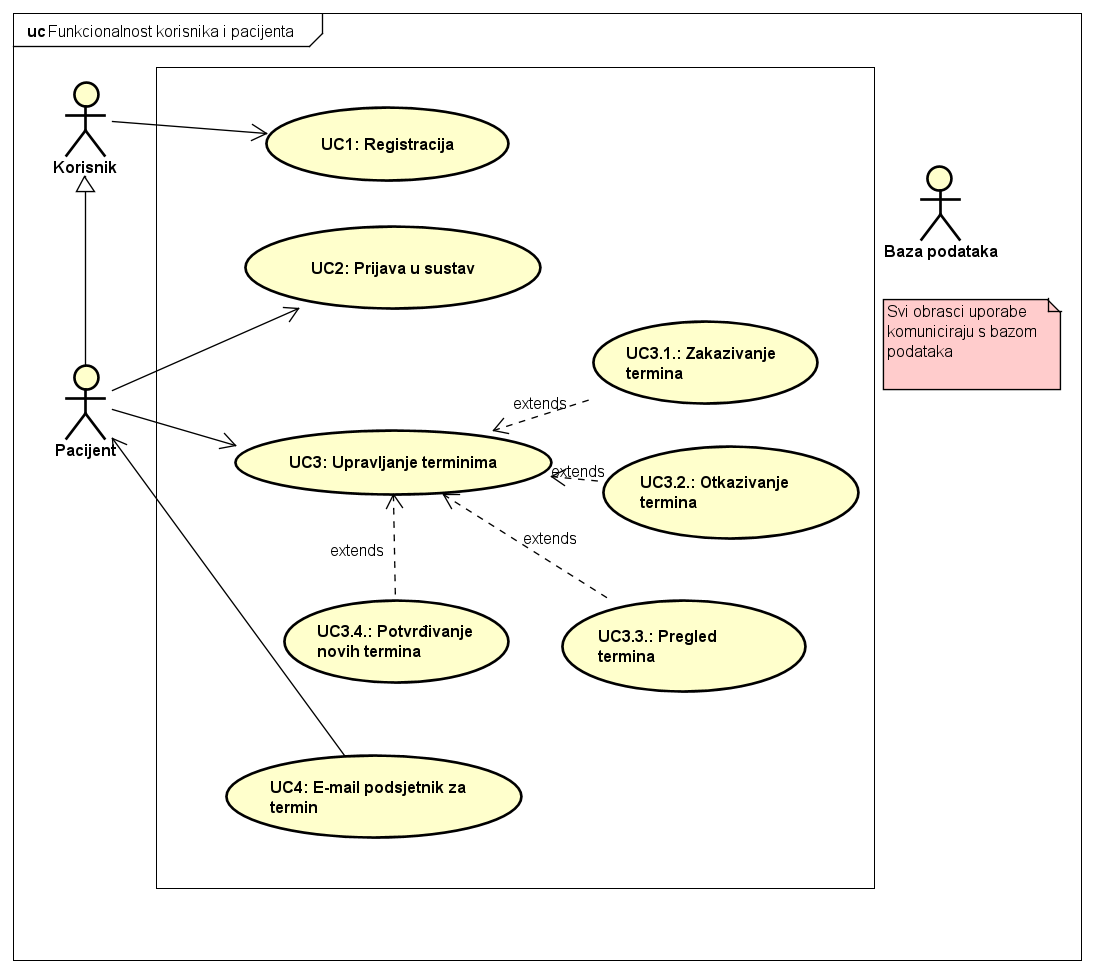
\includegraphics[scale=0.6]{slike/KorisnikIPacijent.PNG} %veličina slike u odnosu na originalnu datoteku i pozicija slike
	\centering
	\caption{Dijagram obrasca uporabe koji prikazuje funkcionalnost korisnika i pacijenta}
	\label{fig:promjene}
\end{figure}

\begin{figure}[H]
	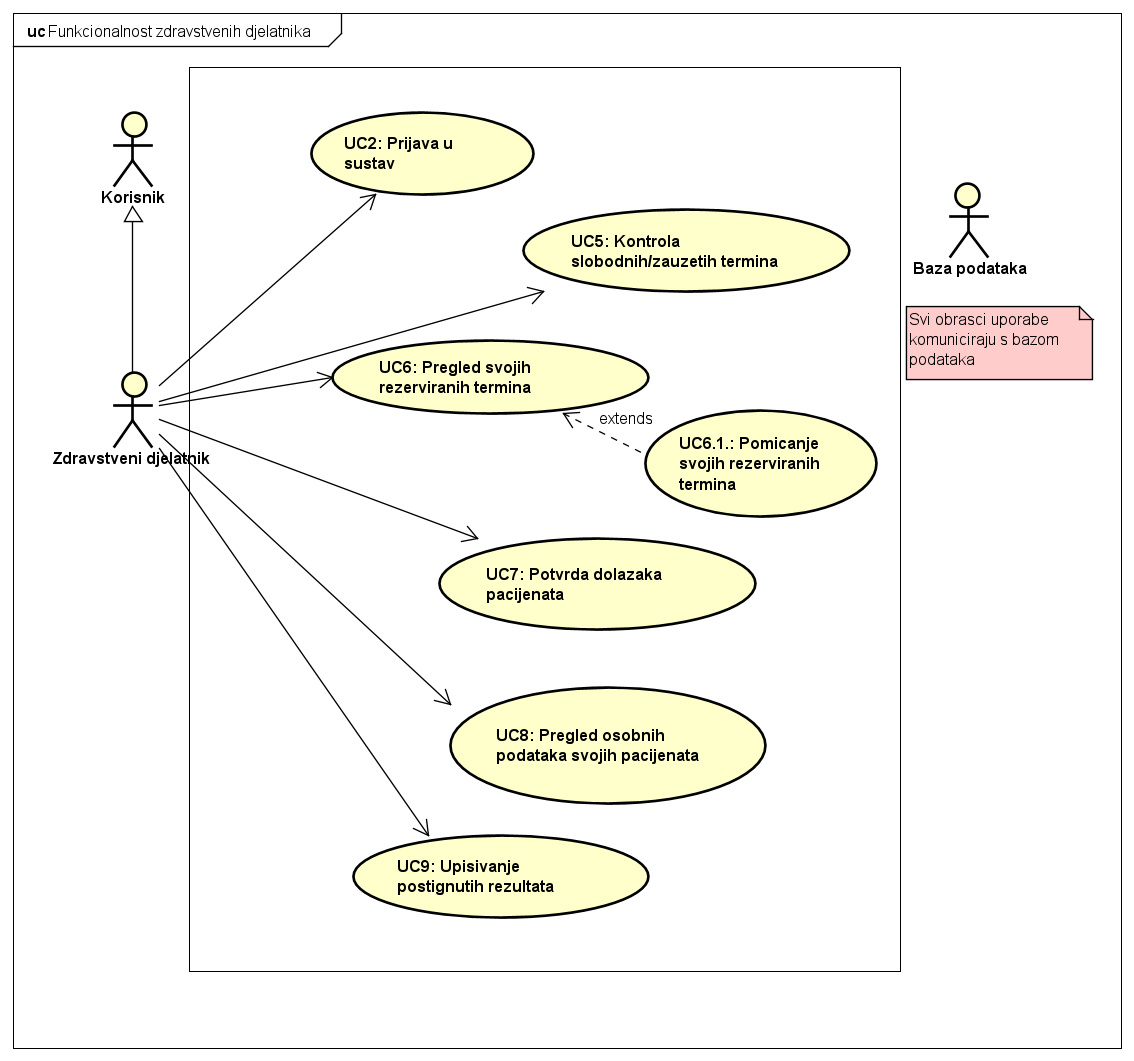
\includegraphics[scale=0.6]{slike/ZdravstveniDjelatnik.PNG} %veličina slike u odnosu na originalnu datoteku i pozicija slike
	\centering
	\caption{Dijagram obrasca uporabe koji prikazuje funkcionalnost zdravstvenih djelatnika}
	\label{fig:promjene}
\end{figure}

\begin{figure}[H]
	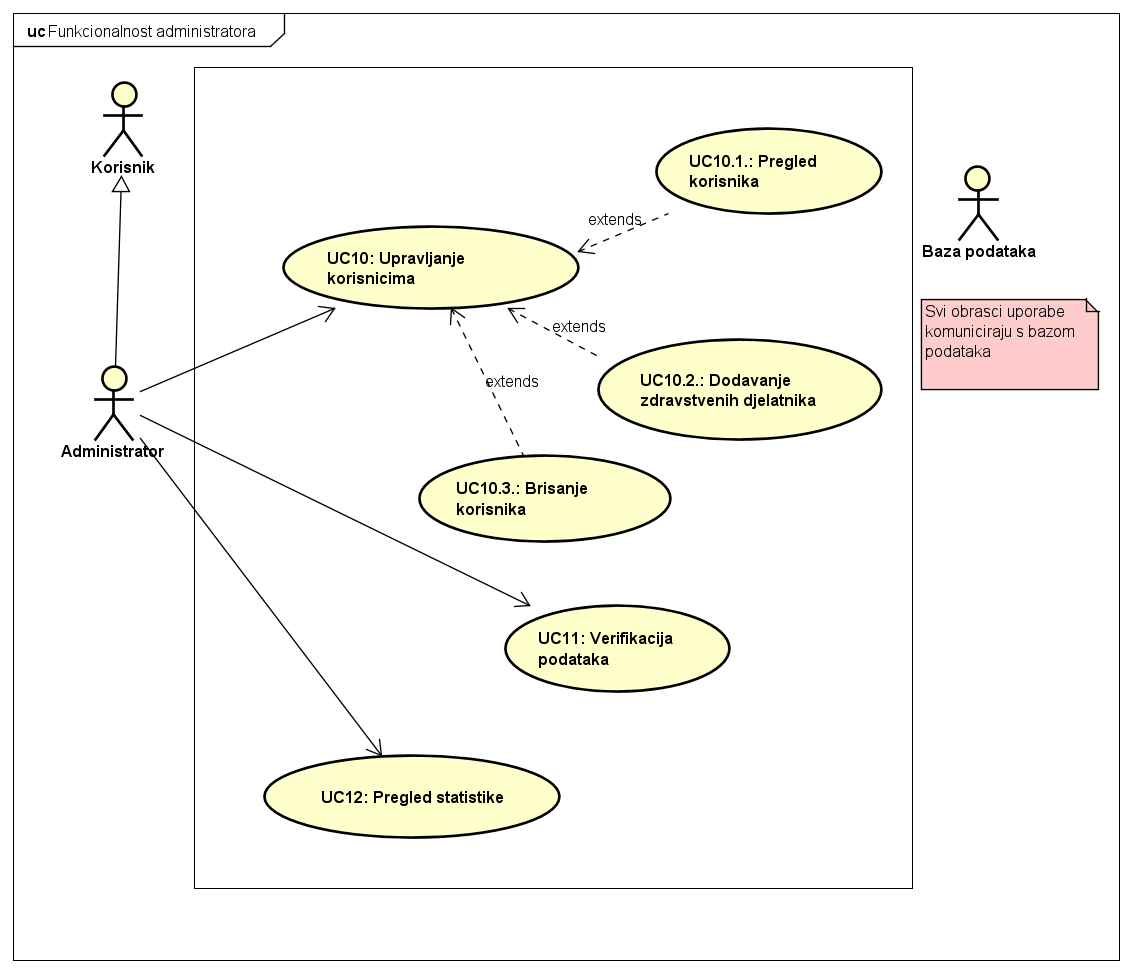
\includegraphics[scale=0.6]{slike/Administrator.PNG} %veličina slike u odnosu na originalnu datoteku i pozicija slike
	\centering
	\caption{Dijagram obrasca uporabe koji prikazuje funkcionalnost administratora}
	\label{fig:promjene}
\end{figure}

\newpage
\subsection{Sekvencijski dijagrami}

\textbf{\text{UC3.1. - Zakazivanje termina}}\\

Korisnik, prijavljen kao pacijent, želi odabrati novi slobodni termin. Poslužitelj dohvaća trenutne termine te korisniku prikazuje kalendar. Pacijent navodi datum i vrijeme kada želi zakazati termin te od strane poslužitelja dobiva pregled svih vlastitih opisa zdravstvenih problema koje je unosio u prošlosti (ako ih ima). Pacijent odabire referencu na ponovljeni opis problema te potvrđuje odabrani termin. Termin se tada sprema u bazu podataka kao nepotvrđeni zahtjev za terminom. Djelatnik dohvaća sve zahtjeve koji odgovaraju njegovoj smjeni te odabire termin koji želi potvrditi. Djelatnik navodi opremu koja mu je potrebna za opisani zdravstveni problem te se vrši provjera dostupnosti opreme. Ako je oprema slobodna, termin se sprema u bazu podataka, djelatnik dobiva potvrdu o spremanju te se pacijentu šalje e-mail o uspješno zakazanom terminu. Ako nema slobodne opreme, djelatnik dobiva listu slobodnih termina u sljedećih tjedan dana te odabire neki od ponuđenih termina, nakon čega se termin sprema u bazu podataka, a djelatnik i pacijent dobivaju prikladnu obavijest.\newline Ako je pacijent unio podatke o novom zdravstvenom problemu, poslužitelj te informacije sprema u bazu podataka. Pacijent potvrđuje odabrani termin te se on sprema kao nepotvrđeni zahtjev za terminom. Postupak je dalje jednak kao i u prijašnjem slučaju - Djelatnik dohvaća sve zahtjeve koji odgovaraju njegovoj smjeni te odabire termin koji želi potvrditi. Djelatnik navodi opremu koja mu je potrebna za opisani zdravstveni problem te se vrši provjera dostupnosti opreme. Ako je oprema slobodna, termin se sprema u bazu podataka, djelatnik dobiva potvrdu o spremanju te se pacijentu šalje e-mail o uspješno zakazanom terminu. Ako nema slobodne opreme, djelatnik dobiva listu slobodnih termina u sljedećih tjedan dana te odabire neki od ponuđenih termina, nakon čega se termin sprema u bazu podataka, a djelatnik i pacijent dobivaju prikladnu obavijest.

\begin{figure}[H]
	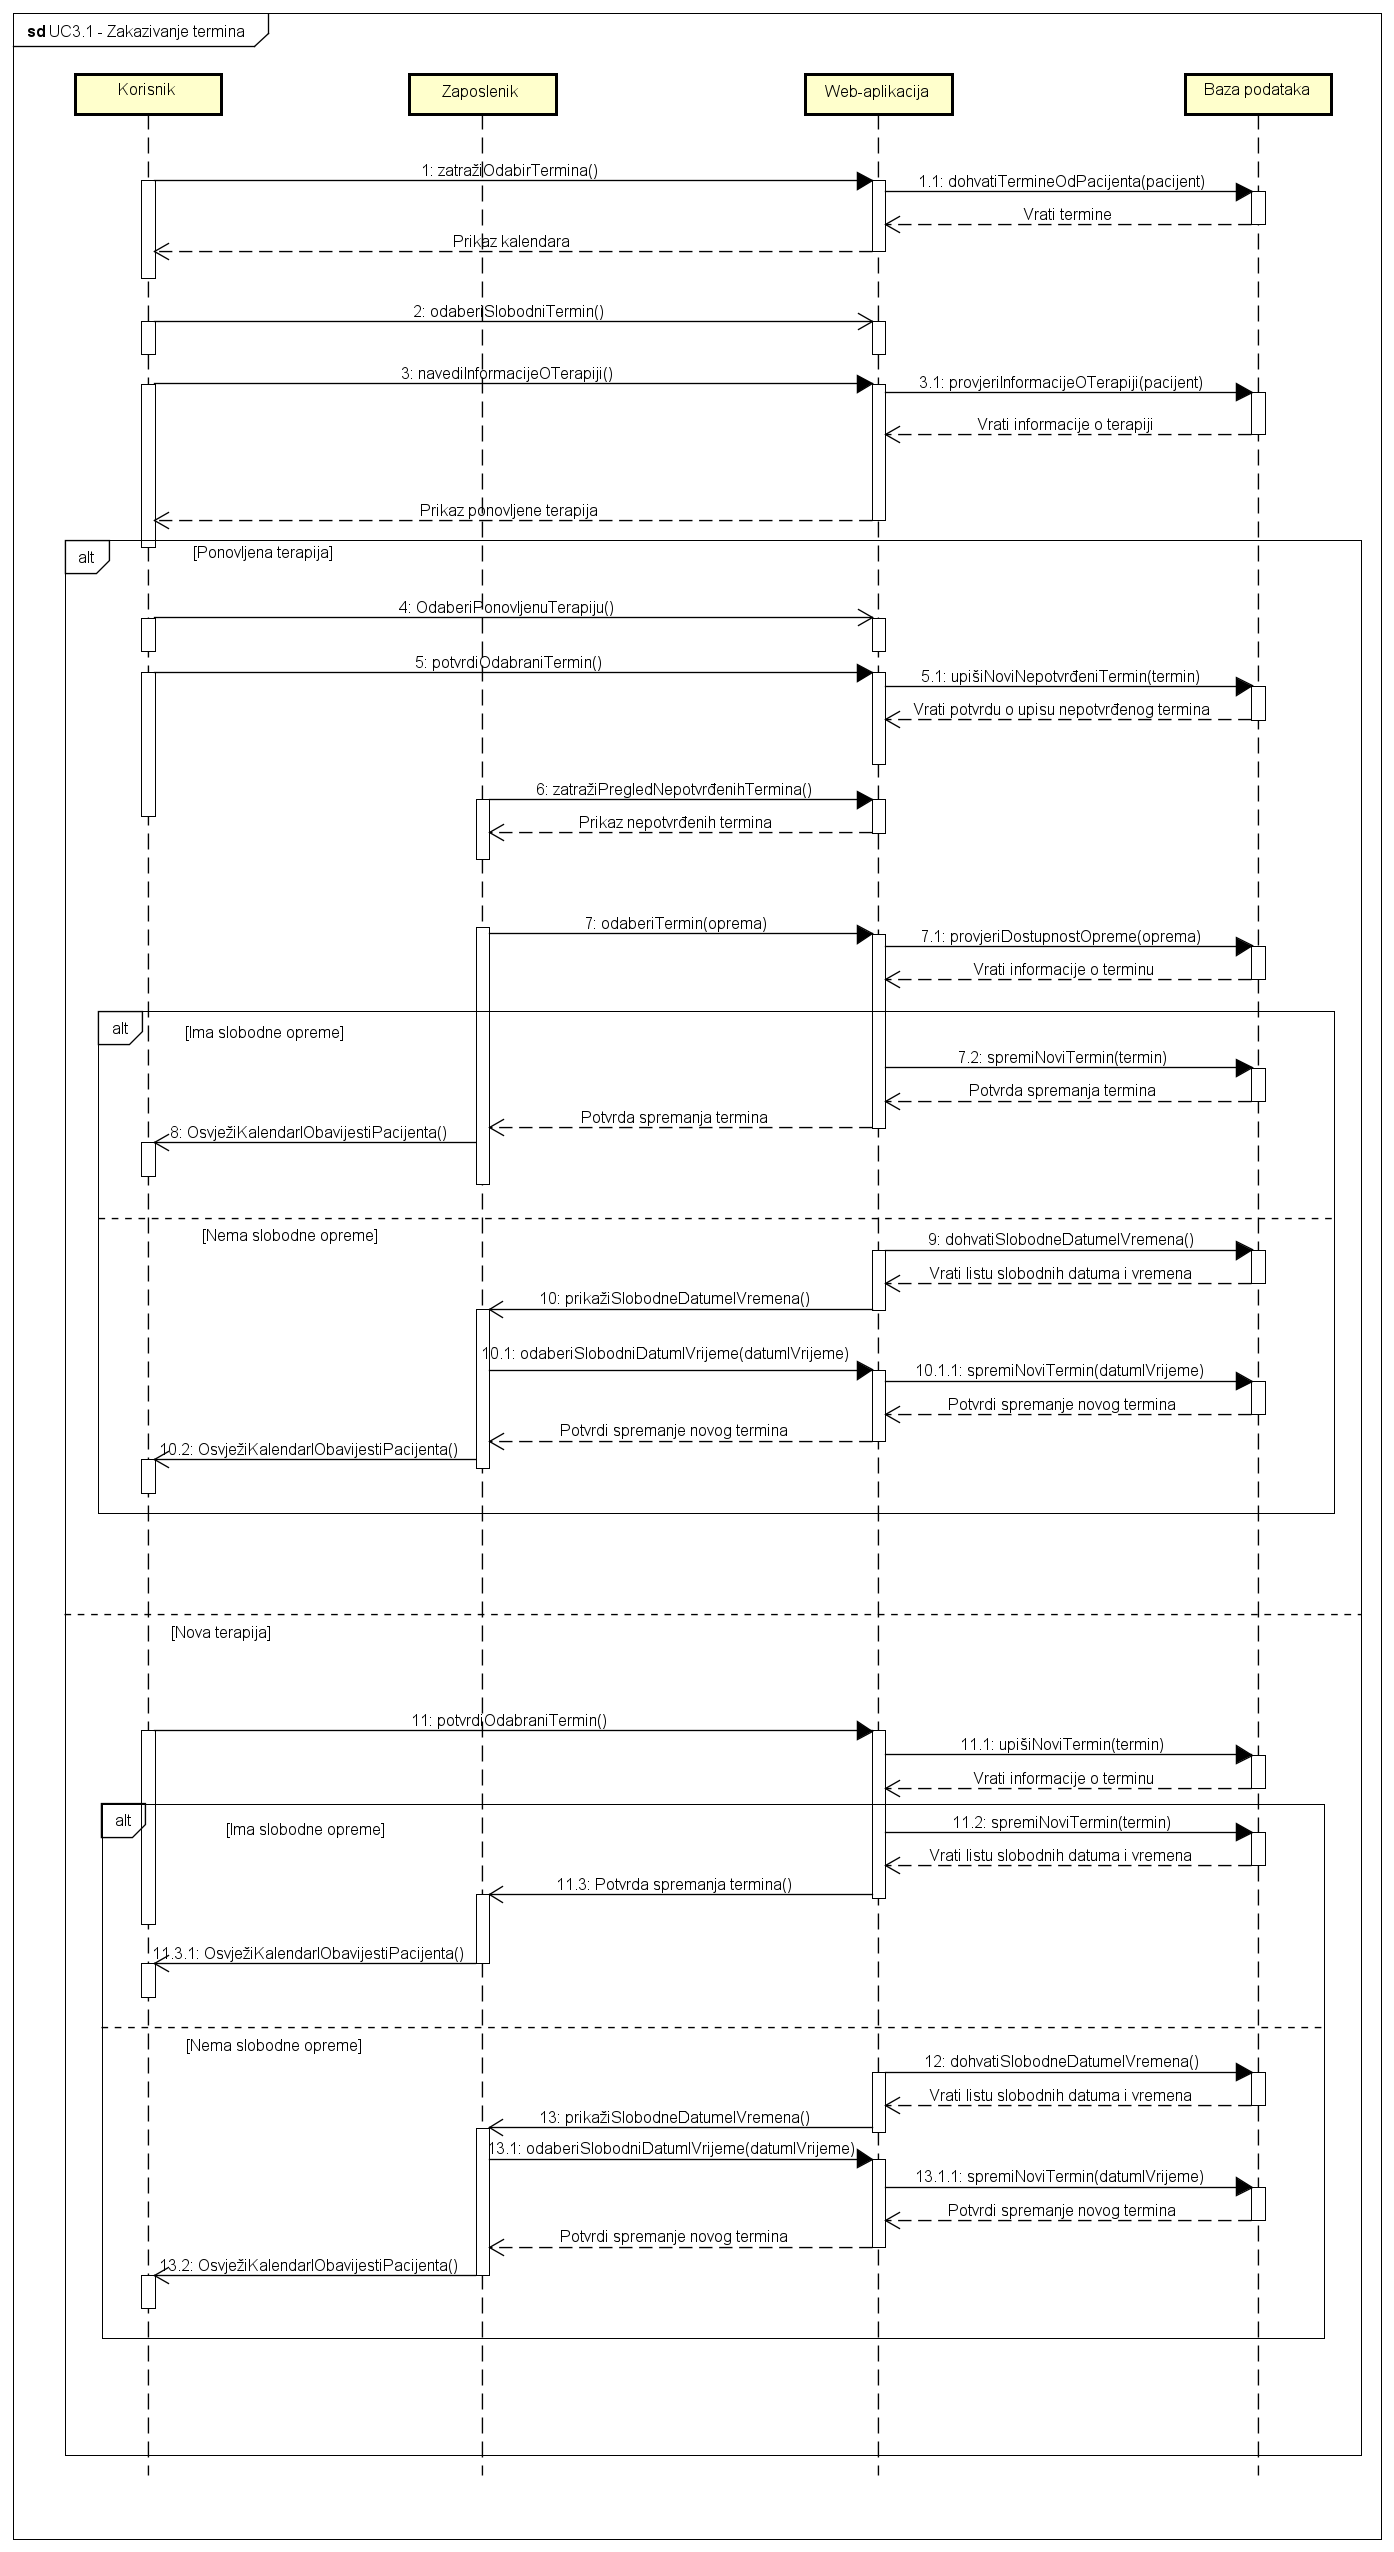
\includegraphics[scale=0.33]{slike/zakazivanjeTerminaUC3.1}
	\centering
	\caption{Sekvencijski dijagram za UC3.1.}
\end{figure}

\newpage

\textbf{\text{UC3.2. - Otkazivanje termina}}\\

Korisnik, prijavljen kao pacijent, želi odabrati termin kako bi ga mogao otkazati. Poslužitelj dohvaća sve zakazane termine od tog pacijenta i prikazuje ih u kalendaru. Pacijent otkazuje odabrani termin. Poslužitelj ispituje ispravnost odabranog termina te ako je on ispravan, briše ga iz baze podataka, osvježava kalendar i šalje e-mail poruku pacijentu. Ako pacijent prekasno pokušava otkazati termin, odnosno ako to čini 24 sata prije zakazanog termina, poslužitelj ne briše termin i šalje odgovarajuću poruku pacijentu.

\begin{figure}[H]
	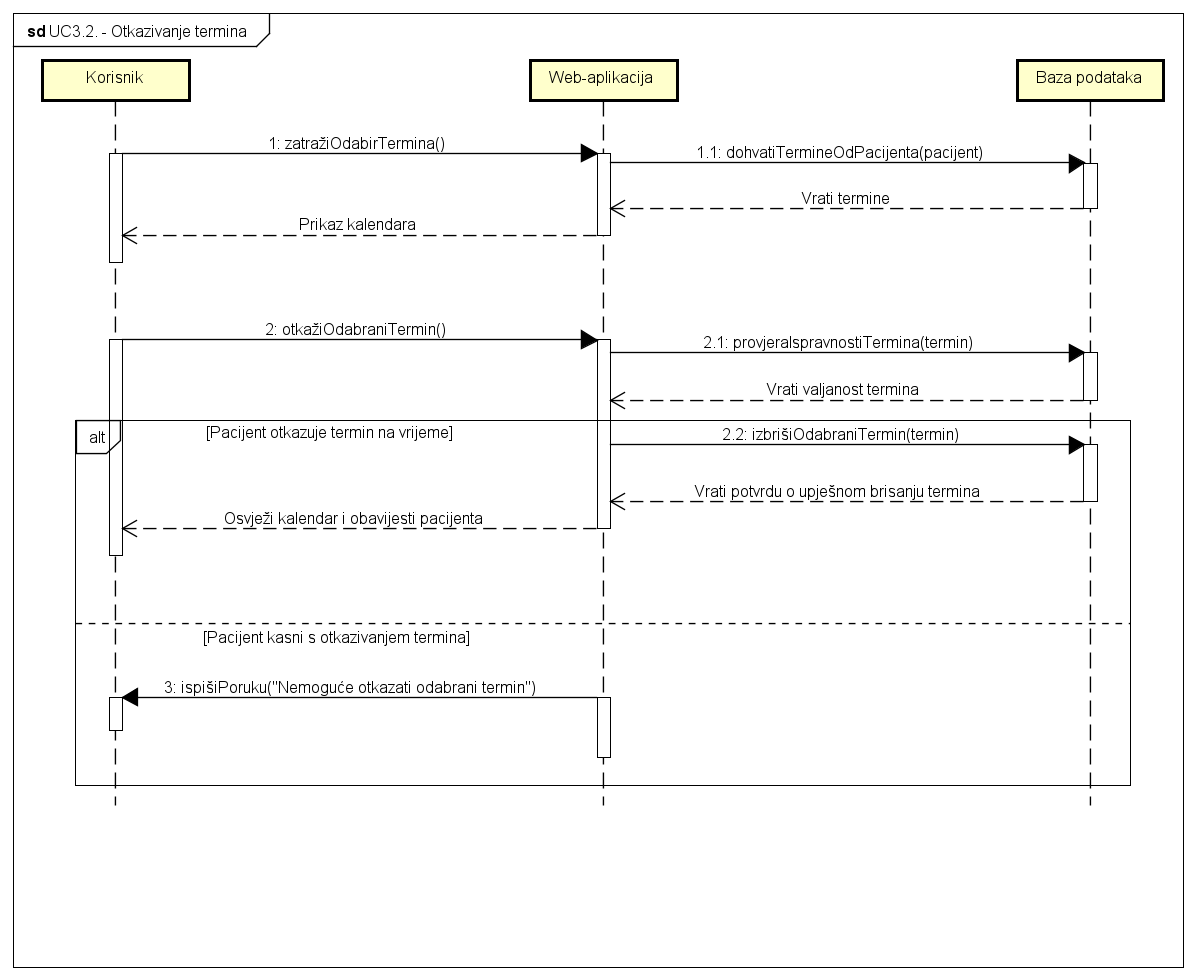
\includegraphics[scale=0.5]{slike/UC3.2_Otkazivanje_termina}
	\centering
	\caption{Sekvencijski dijagram za UC3.2.}
\end{figure}

\newpage

\textbf{\text{UC6.1 - Pomicanje svojih rezerviranih termina}}\\

Korisnik, prijavljen kao zdravstveni djelatnik, želi premjestiti svoje rezervirane termine zbog nemogućnosti njihovog izvršavanja. Poslužitelj dohvaća sve rezervirane termine od zdravstvenog djelatnika te ih prikazuje na kalendaru. Zdravstveni djelatnik odabire sve termine koje bi želio premjestiti. Sljedeći koraci se izvršavaju sve dok se ne obrade svi odabrani termini. Dok se ne dobije potvrda pacijenta, zdravstveni djelatnik odabire opciju otkazivanja trenutno odabranog termina. Poslužitelj ispituje ispravnost odabranog termina te vraća njegovu valjanost. Ako je zdravstveni djelatnik na vrijeme odlučio pomaknuti odabrani termin, on to čini te se pacijentu šalje obavijest o mogućem novom terminu. Ako zdravstveni djelatnik pomiče odabrani termin unutar 24 sata od samoga odabranoga termina, poslužitelj ga u tome onemogućuje. Nakon što pacijent potvrdi suglasnost o novome terminu, zdravstveni djelatnik potvrđuje samu promjenu termina. Poslužitelj dobiva i stari i novi termin te se stari uklanja, a novi dodaje u bazu podataka. Nakon pomicanja termina, zdravstvenom se djelatniku osvježava kalendar.

\begin{figure}[H]
	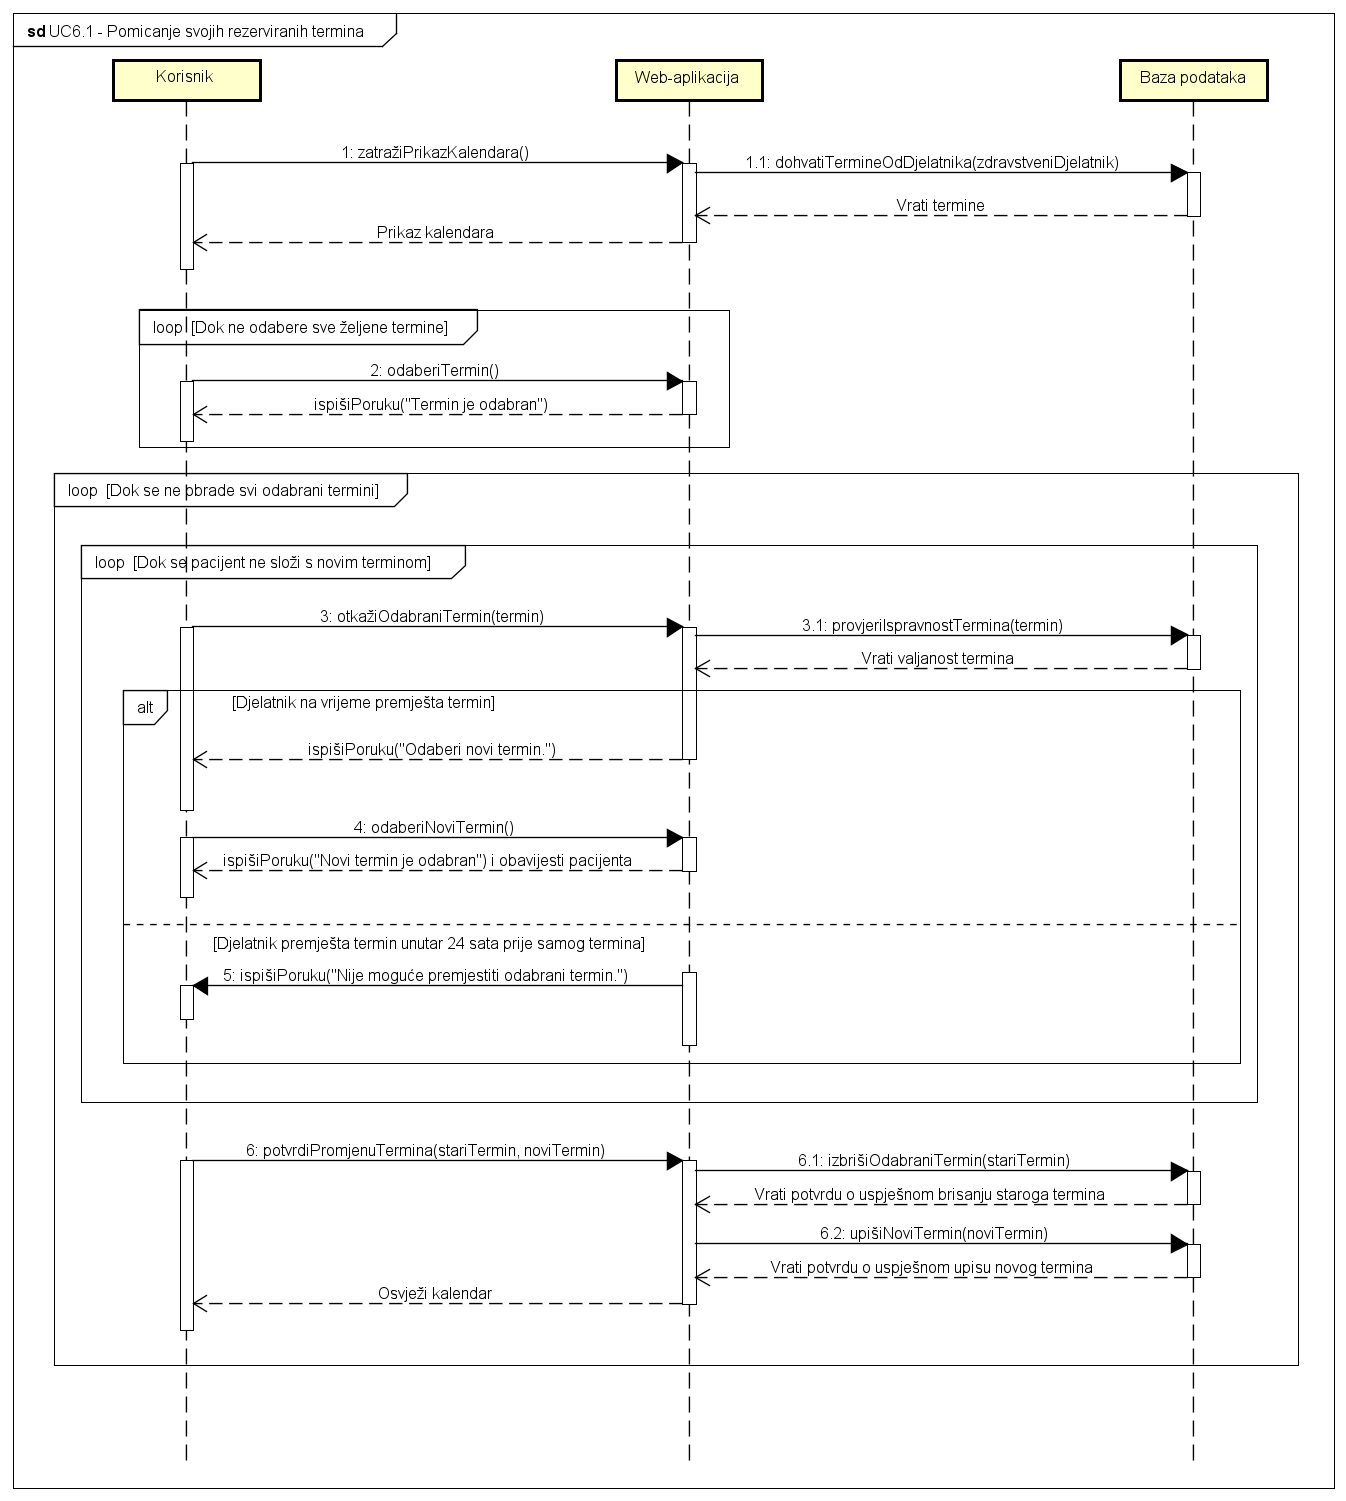
\includegraphics[scale=0.5]{slike/UC6.1_Pomicanje_svojih_rezerviranih_termina}
	\centering
	\caption{Sekvencijski dijagram za UC6.1}
\end{figure}

\section{Ostali zahtjevi}

\begin{packed_item}
	\item Korisničko sučelje mora biti intuitivno i prilagođeno, olakšavajući korisnicima njenu upotrebu
	\item Sustav mora omogućiti istovremeni rad većem broju korisnika
	\item Sustav treba omogućiti brzu i učinkovitu prijavu pacijenata te raspoređivanje termina unutar radnog vremena
	\item Prilikom komunikacije s bazom podataka, svi osobni podaci moraju biti prikladno zaštićeni
	\item Korisnicko sučelje i sustav moraju podržavati hrvatsku abecedu (dijakritičke znakove) pri unosu i prikazu tekstualnog sadrzaja 
	\item Apikacija mora biti oblikovana poštivajući načela objektno-orijentiranog programiranja
	\item Neispravno koristenje korisničkog sučelja ne smije narušiti funkcionalnost i rad sustava
	\item Sustav treba omogućiti obavještavanje pacijenata putem elektroničke pošte o promjenama u rasporedu ili drugim važnim informacijama
	\item Sistemski administrator treba imati potpuni pristup svim podacima i mogućnost definiranja postavki sustava
\end{packed_item}


			 
			 
	